\documentclass{ximera}

\title{Arithmetic Series}

\author{Bart Snapp and Brad Findell}

\begin{document}
\begin{abstract}
We study arithmetic series.
\end{abstract}
\maketitle

\label{A:arithmeticSeries}

In this activity, we explore \emph{arithmetic series}, which are sums of consecutive terms from an arithmetic sequence.

Ms. Nguyen's math class has been looking at ``triangular numbers.''  The first 6 triangular numbers are shown below. 
\begin{image}
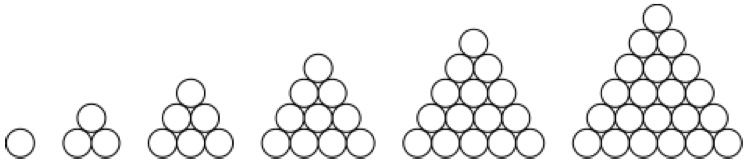
\includegraphics{graphics/triangularNumbers}
\end{image}
%\fixnote{Maybe start this problem without help.  Need an original graphic.}

\begin{problem}
Blair wanted to find the $551^{st}$ triangular number.  She used a table and looked for a pattern in the \emph{sequence of partial sums}:  $1, 1+2, 1+2+3, \dots$.  Help her finish her idea.  
\end{problem}

\begin{problem}
Kaley realized the the $551^{st}$ triangular number would be the sum 
\[
1+2+3+4+\dots+548+549+550+551
\]
She started pairing the first with the last number; the second with the second-to-last; the third with the third-to-last; and so on.  She saw that the averages are always the same.  Help her finish her idea.  
\end{problem}

\begin{problem}
Ali begin by writing out the sum forward and backward and follows:  
\[
\begin{array}{c@{ + }c@{ + }c@{ + }c@{ + }c@{ + }c@{ + }c@{ + }c@{ + }c@{ + }c@{ + }c@{ + }c@{ + }c}
1 & 2 & 3 & 4 & 5 & 6 & \cdots & 546 & 547 & 548 & 549 & 550 & 551 \\
551 & 550 & 549 & 548 & 547 & 546 & \cdots & 6 & 5 & 4 & 3 & 2 & 1 
\end{array}
\]
Help her finish her idea.  Be sure to explain clearly what happens ``in the dots.''  Does it matter whether there are an even or an odd number of terms?  
\end{problem}

\begin{problem}
Cooper was interested in a different triangular number and drew the following picture:   
\begin{image}
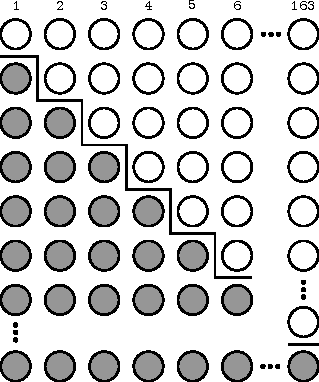
\includegraphics{graphics/sum1.pdf}
\end{image}
Which triangular number was he finding?  Help him finish his idea.  Be sure to explain clearly what 
happens ``in the dots.'' 
\end{problem}


\begin{problem}
Sum the numbers:  
\[
106 + 112 + 118 + \dots + 514
\]
\end{problem}

\begin{problem}
Sum the numbers:
\[
2.2 + 2.9 + 3.6 + 4.3 + \dots + 81.3
\]
\end{problem}


\begin{problem}
Suppose you have an arithmetic sequence beginning with $a$, with a constant difference of $d$ and with $n$ terms.  
\begin{enumerate}
\item What is the $n^{th}$ term of the sequence?  
\item Use dots to write the series consisting of the first $n$ terms of this sequence.
\item Find the sum of this series.  
\end{enumerate}
\end{problem}
\end{document}

